\documentclass[10pt,twocolumn,letterpaper]{article}

\usepackage{iccv}
\usepackage{times}
\usepackage{epsfig}
\usepackage{graphicx}
\usepackage{amsmath}
\usepackage{amssymb}
\usepackage{dsfont}
\usepackage{xcolor}

 \usepackage{caption}
 \usepackage{subcaption}
\graphicspath{ {./images/} }

% Include other packages here, before hyperref.

% If you comment hyperref and then uncomment it, you should delete
% egpaper.aux before re-running latex.  (Or just hit 'q' on the first latex
% run, let it finish, and you should be clear).
\usepackage[pagebackref=true,breaklinks=true,letterpaper=true,colorlinks,bookmarks=false]{hyperref}

% \iccvfinalcopy % *** Uncomment this line for the final submission

\def\iccvPaperID{****} % *** Enter the ICCV Paper ID here
\def\httilde{\mbox{\tt\raisebox{-.5ex}{\symbol{126}}}}

% Pages are numbered in submission mode, and unnumbered in camera-ready
\ificcvfinal\pagestyle{empty}\fi
\begin{document}

%%%%%%%%% TITLE
\title{Youtube2Story: Unsupervised Joint-Representation of Instructional Videos}

\author{First Author\\
Institution1\\
Institution1 address\\
{\tt\small firstauthor@i1.org}
% For a paper whose authors are all at the same institution,
% omit the following lines up until the closing ``}''.
% Additional authors and addresses can be added with ``\and'',
% just like the second author.
% To save space, use either the email address or home page, not both
\and
Second Author\\
Institution2\\
First line of institution2 address\\
{\tt\small secondauthor@i2.org}
}

\maketitle
%\thispagestyle{empty}


%%%%%%%%% ABSTRACT
\begin{abstract}
   The ABSTRACT
\end{abstract}

%%%%%%%%% BODY TEXT
% !TEX root = recipeUnderstanding.tex

\section{Introduction}
Human communication takes many forms, including language and vision. For instance, explaining ``how-to'' perform a certain task can be communicated via language (e.g., Do-It-Yourself books) as well as visual (e.g., instructional YouTube videos) information. Regardless of the form, such human-generated communication is generally structured and has a clear beginning, end, and a set of steps in between. Parsing such communication into its semantic steps is the key to understand human activities.

%% AMIR: paragraph Could be removed
Language and vision provide different, but correlating and complementary information. Challenge lies in that both video frames and language (from subtitles generated via Automatic Speech Recognition) are only a noisy, partial observation of the actions being performed. However, the complementary nature of language and vision gives the opportunity to understand the activities only from these partial observations. In this paper, we present a unified model, considering both of the modalities, in order to parse human activities into activity steps with no form of supervision other than requiring videos to be the same category (\eg all cooking eggs, changing tires etc.).

%

%requires us to model them jointly. We present a unified model, learnt in a fully unsupervised manner, in order to jointly use these two modalities.

% Furthermore they are
% We utilize these two modalities (video frames and imperfect automatically generated subtitles) in a unified manner in our framework;
% We qualitatively and quantitatively argue that a joint inference is crucial for a successful semantic parsing, particularly when no supervision is employed.


%  the proposed approach on instructional videos from YouTube (\eg, ``Making panckage'', ``How to tie a bow tie'') as they typically have clear steps and provide concrete grounds for demonstrating a semantically meaningful parsing. These videos are often long and manifest a high intra-class variability yet the underlying steps remains well-defined and structured, similar to almost all human communications.

\begin{figure}[h!]
  \includegraphics[width=0.48\textwidth]{Figure_1_flattened}
  \caption{Given a large video collection (frames and subtitles) of an instructional category (\eg How to cook an ommelette?), we discover activity steps (\eg crack the eggs). We also parse the videos based on the discovered steps.}
  \label{teaser}
  \vspace{-5mm}
\end{figure}


The key idea in our approach is the observation that the large collection of videos, pertaining to the same activity class, typically include only a few objective activity steps, and the variability is the result of exponentially many ways of generating videos from activity steps through subset selection and time ordering. We study this construction based on the large-scale information available in YouTube in the form of instructional videos  (\eg, ``Making panckage'', ``How to tie a bow tie''). Instructional videos have many desirable properties like the volume of the information (e.g., YouTube has 281.000 videos for \emph{"How to tie a bow tie"}) and a well defined notion of activity step.  However, the proposed parsing method is applicable to any type of videos as long as they are composed of a set of steps.

%I think the story line idea is not that strong anymore, we are discovering and parsing
The output of our method can be seen as the semantic ``storyline'' of a rather long and complex video collection (see Fig. \ref{teaser}). This storyline provides what particular steps are taking place in the video collection, when they are occurring, and what their meaning is (\emph{what-when-how}). This method also puts videos performing the same overall task in common ground and capture their high-level relations.

%, and therefore, provide a \emph{categorical} storyline as well.

In the proposed approach, given a collection of videos, we first generate a set of language and visual atoms. These atoms are the result of relating object proposals from each frame as well as detecting the frequent words from subtitles. We then employ a generative \emph{beta process mixture model}, which identifies the activity steps shared among the videos of the same category based on a representation using learned atoms. Although we do not explicity enforce this steps to be semantically meaningful, our results highly correlate with the semantic steps. In our method, we do neither use any spatial or temporal label on actions/steps nor any labels on object categories. We later learn a Markov language model to provide a textual description of the activity steps based on the language atoms it frequently uses.

%This work is the first to discover activity steps for a complex video collection with no supervision over activity steps and/or objects. We are also the first to approach this problem in a multimodal (joint language and vision) manner.
%In addition, our method is capable of providing a caption describing the steps; our approach to captioning is fundamentally different from the existing video/image-to-text work in two aspects: 1) the captions are generated without any supervised caption-clip pairs, 2) our captions are \emph{descriptions} of the semantic steps, yet they are inferred from \emph{narrations}. This is different from the existing captioning work as their reference data is descriptive of the visual information, while the narration over videos often provides complementary information to the visuals and is not necessarily descriptive.

\section{Related Work}
\paragraph{Video Summarization}
Summarizing an input video as a sequence of keyframes (static) or as a sequence of video clips (dynamic) is useful for both multi-media search interfaces and retrieval purposes. Early works in the area are summarized in \cite{vidAbstraction} and mostly focus on choosing key-frames for visualization. Idea of choosing key-frames is also extended by using the video tags by Hong et al\cite{beyondSearch} and using the spatio-temporal information by Gygli et al.\cite{createSum}.

Summarizing videos is crucial for ego-centric videos since the ego-centric videos are generally long in duration. There are many works which succesfully segment such videos in to a sequence of important shots \cite{lee2012discovering, lu2013story}; however, they mostly rely on specific features of ege-centric videos. Rui et al. \cite{rui2000automatically} proposed another dynamic summarization method based on the excitement in the speech of the reporter. Due to their domain specific designs, these algorithms are not applicable to the general instructional videos.

%http://www.sangminoh.org/Publications_files/Oh2012bmvc_videography.pdf --> learn atomic representations and do not do a segmentation
Same idea is also applied to the large image collecitons by recovering the temporal ordering and visual similarity of images \cite{storyGraph}. This image colelctions are further used to choose important view points for video key-frame selection by Khosla et al.\cite{khosla2013large}. And further extended to video clip selection by Kim et al\cite{kim2014joint} and Potapov et al.\cite{potapov2014category}. Although they are different from our approach since they do not use any high-level semantic information or the language information, we experimentally compare our method with them.


\paragraph{Understanding Multi-Modal Information:} Captioning Work, What are you talking about? Text-to-Image Coreference(urtasun), Bringing Semantics Into Focus Using Visual Abstraction, Learning the Visual Interpretation of Sentences Zitnick (parikh) clip art to understand spatial relations of objects and language, Improving Video Activity Recognition using Object Recognition and Text Mining Motwani uses captions and object detectors to learn activities automatically. Grounded Language Learning from Video Described with Sentences (yu) improve semantic parsing using object/activity detectors. Matching Words and Pictures, A Sentence is Worth a Thousand Pixels, Connecting Modalities: Semi-supervised Segmentation and Annotation of
Images Using Unaligned Text Corpora, Grounded Compositional Semantics
for Finding and Describing Images with Sentences, Multimodal Neural Language Models, Every Picture Tells a Story: Generating Sentences from Images, m2Text: Describing Images Using 1 Million
Captioned Photographs

\paragraph{Activity Detection/Recognition:}

\paragraph{Recipe Understanding}
Following the interest in community generated recipes in the web, there have been many attempts to automatically process recipes. Recent methods on natural language processing \cite{cookingSemantics,logicRecipe} focus on semantic parsing of language recipes in order to extract actions and the objects in the form of predicates. Tenorth et al.\cite{logicRecipe} further process the predicates in order to form a complete logic plan. Mori et al.\cite{flowGraph} also learns the relations of the actions in terms of a flow graph with the help of a supervision. The aforementioned approaches focus only on the language modality and they are not applicable to the videos. We have also seen recent advances \cite{beetz,cookie} in robotics which uses the parsed recipe in order to perform cooking tasks. They use supervised object detectors and report a succesfull autonomous cooking experiment. In addition to the language based approaches, Malmaud et al.\cite{alignment} consider both language and vision modalities and propose a method to align an input video to a recipe. However, it can not extract the steps/actions automatically and requires a ground truth recipe to align. On the contrary, our method uses both visual and language modalities and extracts the actions while autonomously constructing the recipe. There is also an approach which generates multi-modal recipes from expert demonstrations \cite{photoshop}. However, it is developed only for the domain of \emph{teaching user interfaces} and are not applicable to the videos.

% !TEX root = recipeUnderstanding.tex

\vspace{-1mm}
\section{Overview}
\label{sec:overview}
\vspace{-1mm}

%\begin{figure}[h]
%  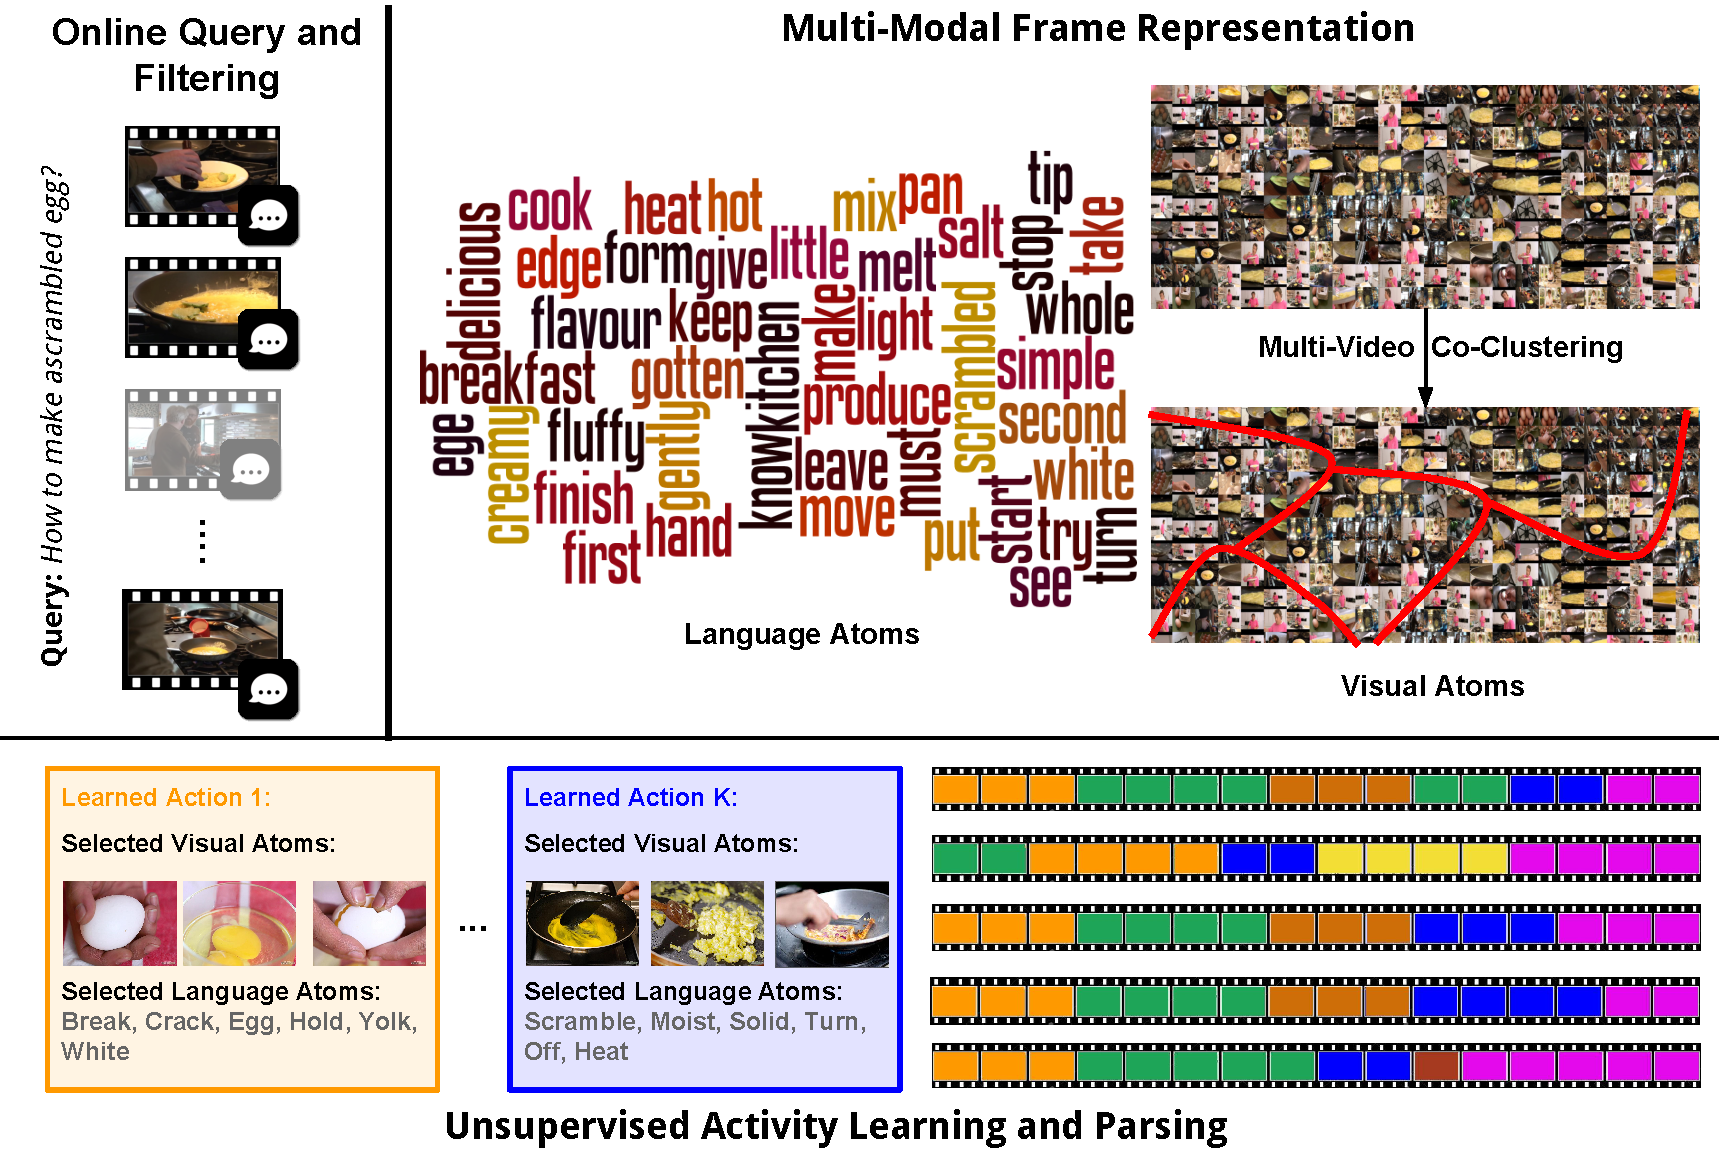
\includegraphics[width=0.5\textwidth]{algor}
%  \caption{Components of our recipe understanding method. \textbf{Query:} We query the YouTube for top 100 \emph{How To} videos and filter the outliers; \textbf{Framewise Representation:} We automatically extract object clusters and salient word in order to find multi-modal representation of each frame. \textbf{Unsupervised Activity Detection:} We jointly cluster videos in order to learn activities/steps related to the recipe.}
%\label{fig:overview}
%\end{figure}

Given a large video-collection, our algorithm starts with learning a set of visual and language atoms which are further used for representing multimodal information (Section~\ref{atoms}). These atoms are designed in a way to be likely to correspond to the mid-level semantic concepts like actions and objects. In order to learn visual atoms, we generate object proposals and cluster them into mid-level atoms. Whereas, for the language atoms we simply find the salient and frequent words in the subtitles. After learning the atoms, we represent the multi-modal information in each frame based on the occurrence statistics of the atoms (Section~\ref{atoms}); Given the series of multi-modal frame representations, we discover set of clusters occurring over multiple videos using a non-parametric Bayesian method (Section~\ref{learning}). We expect these clusters to correspond to the activity steps which construct the high level activities. Our empirical results confirms this as the resulting clusters significantly correlates with the activity steps.

%In , we explain how we learn the language and visual atoms. Then, we explain the multi-modal representation of the frames in . Finally we explain how do we discover activity steps in 


%In this section, we explain the high-level components of our method which we visualize in Figure~\ref{fig:overview}. Our proposed method consists of three major components; \textbf{(1) Online query and filtering:} Our system starts with querying the YouTube with an \emph{How to} question, and records the top 100 resulting videos. In order to detect the similarity of the videos quickly, we also process the text descriptions and eliminate outliers. \textbf{(2) Frame-wise multi-modal representation:} In order to semantically represent the spatio-temporal information in the videos, we process both the visual and language content of each video. We extract the region proposals and jointly cluster them to detect semantic visual objects. We also detect the salient words of the subtitles. Finally, we epresent the each frame in terms of the resulting objects and the salient words. \textbf{(3) Unsupervised joint clustering:} After describing the each frame by using both language and visual cues, we apply 


\section{Semantic Multi-Modal Frame Representation}
\subsection{Learning Atoms to Represent Multi-Modal Data}
We represent each frame in our video set as a distribution over set of language and visual atoms. Language atoms are the salient words detected by using a tf-idf like measure, and the visual atoms are found via clustering over object proposals which we extract from frames. We explain the details of finding the atoms and representing the frames in the subsequent sections.
\subsubsection{Learning Language Atoms}
In order to detect salient words, we use tf-idf like measure. For each recipe, we concatanate all subtitles into a single term corpus. As a document corpus, we use all the words extracted from all recipes. Moreover, we compute the tf-idf as $tfidf(w,d,D)=f_{w,d} \times \log \frac{N}{n_{w}}$ where $w$ is the word, $d$ is the corpus of the recipe and $f_{w,d}$ is the frequency of the word in the recipe. Moreover, $N$ represents the total number of videos in all recipes and $n_{w}$ is the number of videos whose subtitle include the word $w$. After computing the tf-idf, we sort all words with their tf-idf values and choose top $K$ words as set of salient words.
\subsubsection{Learning Visual Atoms}
In order to learn visual atoms, we initially generate object proposals from each frame of each videos.
\paragraph{Generating Framewise Object Proposals}
\paragraph{Joint Proposal Clustering to Detect Visual Objects}
\begin{figure}[ht]
  \begin{subfigure}[b]{0.23\textwidth}
\includegraphics[width=\textwidth]{im0.png}
%\caption{Cluster 1}
\end{subfigure}
~
\begin{subfigure}[b]{0.23\textwidth}
\includegraphics[width=\textwidth]{im4.png}
%\caption{Cluster 2}
\end{subfigure}
\begin{subfigure}[b]{0.23\textwidth}
\includegraphics[width=\textwidth]{im5.png}
\end{subfigure}
~
\begin{subfigure}[b]{0.23\textwidth}
\includegraphics[width=\textwidth]{im7.png}
\end{subfigure}

\begin{subfigure}[b]{0.23\textwidth}
\includegraphics[width=\textwidth]{im8.png}
\end{subfigure}
~
\begin{subfigure}[b]{0.23\textwidth}
\includegraphics[width=\textwidth]{im10.png}
\end{subfigure}
\caption{Randomly selected images of randomly selected clusters learned for \emph{How to boil an egg?}}
\end{figure}
\subsection{Multi-Modal Representation via Learned Atoms}

\section{Unsupervised Activity Representation}
\label{basics}
Here we explain the generative model which we use in order to jointly learn the activities from videos. We start with explaining the basic notation we use in the model. We denote the $t^{th}$ frame of the $i^{th}$ video as $I^i_t$ and its subtitle as $L^i_t$. Moreover, we note the extracted frame representation as $y^i_t$. We model our algorithm based on activities and the note the activity of the $t^{th}$ frame of the $i^{th}$ video as $z^i_t$. Since our model is non-parametric, number of activities are not fixed and $z^i_t \in \mathcal{N}$.

\paragraph{Frame:} Representation of each frame is computed as the occurence vector over the detected language and visual atoms. Formally, frame $y^i_t$ is represented as $y^i_t=[y^{i,l}_t,y^{i,v}_t]$ such that $k^th$ entry of the $y^{i,l}_t$ is $1$ if the frame as language atom $k$ and $0$ otherwise. $y^{i,l}_t$ is also a binary vector similarly defined over visual atoms. We consider $y^i_t$ as the observed variable and consider the underlying activity label as the hidden state $z^i_t$. A sample state is visualized in the Figure \ref{visFrame}.

\begin{figure}
  \caption{Visualziation of the representation of the Frame.}
\end{figure}

\paragraph{Activity:} We represent each activity as a Bernoulli distribution over the visual and language atoms. In other words, each frame's representation $y^i_t$ is sampled from its activity distribution as $y^i_t|z^i_t=k \sim Ber(\Theta_k)$. For the sake of clarity, we sample the $\Theta$ from its conjugate distribution \emph{Beta distribution}.

In the following sections, we exlpain how these models can be jointly learned and inferred by using the Beta Process Hidden Markov Models.
s
\subsection{Beta Process Hidden Markov Model}
For joint understanding of the time-series information, Fox et al.\cite{foxBPHMM} proposed the Beta Process Hidden Markov Models (BP-HMM) using the Indian Buffet Process\cite{ibp} of time-series sequences over features. It assumes that there exist a set of features(activities in our case) which can explain the behaviour of all time-series data (all videos in our case). Each time-series data exhibits a subset of available features. This setup is similar to Hughes et al.\cite{npActivity}. However, we differ in the choices of the underlying distributions since we based our model on semantic multi-modal information.

In our model, each video $i$ chooses a set of activities through a activity vector $\mathbf{f^i}$ such that $f^i_k$ is $1$ if $i^th$ video has activity $k$, 0 otherwise. When the feature vectors of all videos in the courpus is concatanated, it becomes an activity matrix $\mathbf{F}$ such that $i^th$ row of the $\mathbf{F}$ is the activity vector $\mathbf{f^i}$. Moreover, each feature $k$ also has an activity frequency $b_k$  and a distribution parameter $\Theta_k$. Distribution parameter $\Theta_k$ is the Bernoulli distribution as explain in the Section \ref{basics}. Moreover, its base distribution ($B_0$) is \emph{Beta random variable} since it is the conjugate of Bernoulli.
 Moreover, in this setting, the activity paremeters $\Theta_k$ and $b_k$ follow the \emph{beta process} as;
\begin{equation}
  B|B_0,\gamma,\beta \sim \text{BP}(\beta,\gamma B_o), B=\sum_{k=1}^\infty b_k \delta_{\Theta_k}
\end{equation}
where $B_0$ and the $b_k$ are determined by the underlying poisson process \cite{hbp} and the feature vector is determined as independent Bernoulli draws as $f_{k}^i \sim Ber(b_k)$. After marginilizing over the $b_k$ and $\Theta_k$, this distribution is shown to be equivalent to Indian Buffet Process \cite{bpibp}. Where videos are customers and activities are dishes in the buffet. The first video chooses a $\text{Poisson}(\gamma)$ unique dishes. The following video $i$ chooses previously sampled activity $k$ with probability $\frac{m_k}{i}$ proportional to number of videos ($m_k$) chosen the activity $k$, and it also chooses $\text{Poisson}(\frac{\gamma}{i})$ new activities. Here, $\gamma$ controls the number of active features in each video and $\beta$ controls the likelihood of the features getting shared by multiple videos.

After each video chooses a subset of activities, we model the videos as an Hidden Markov Model (HMM) over the selected videos. Each frame has the hidden state activity id($z^i_t$) and we observe the binary representation $y^i_t$. Since we model each activity as a Bernoulli distribution, the emmition probabilities follow the Bernoulli distribution as $p(y^i_t|z^i_t)=Ber(\Theta_{z^i_t})$. Following the construction of the Fox et al.\cite{foxBPHMM}, we sample the transition probabilities from a normalized Gamma distribution. For each video $i$, we sample a Gamma random variable for the transition between activity $j$ and activity $k$ if both of the activities are included by the video (if $f^i_k$ and $f^i_j$ are both $1$). After sampling these random variables, we normalize them to have proper transition probabilities. This procedure can be represented formally as
\begin{equation}
  \eta_{j,k}^i \sim Gam(\alpha+\kappa \delta_{j,k},1), \quad \pi_j^i = \frac{\eta^i_j \circ f^i}{\sum_k \eta^i_{j,k} f^i_k}
\end{equation}
Where $\kappa$ is the persistence parameter promoting self state transitions to have more coherent temporal bounderies, $\circ$ is the element-wise product and $\pi^i_j$ is the transition probabilities in video $i$ from state $j$ to all states in the form of a vector.

This model is also presented as a graphical model in Figure \ref{bphmmo}
\begin{figure}[h!]
  \includegraphics[width=0.5\textwidth]{plate}
  \caption{\textbf{Graphical model for BP-HMM:}Some explanation.}
  \label{bphmmo}
\end{figure}


\subsection{Gibbs sampling for BP-HMM}
We employ Markov Chain Monte Carlo (MCMC) method for learning and inference of the BP-HMM. We base our algorithms on the MCMC procedure proposed by Fox et al.\cite{foxBPHMM}. It marginilizes over blah and blah and sample blah and blah. For faster convergence, we also utilize a series of data driven samplers. Here we only discuss the proposed data driven samplers and move the details of the remainin samplers to the Supplementary Material.

\paragraph{Data-Driven Sampler1}
\paragraph{Data-Driven Sampler2}

\section{Experiments}
In order to experiment the proposed method, we first collected a dataset (details in Section~\ref{dataset:sec}). We labelled small part of the dataset with frame-wise activity step labels and used the resulting set as an evaluation corpus. Neither the set of labels, nor the temporal boundaries are exposed to our algorithm since the set-up is completely unsupervised. We evaluate our algorithm against the several unsupervised clustering baselines and state-of-the-art algorithms from video summarization literature which are applicable.
\subsection{Dataset}
\label{dataset:sec}
We use WikiHow\cite{wikiHow} in order to obtain the top100 queries the internet users are interested in and choose the ones which are directly related to the physical world. In other words, we ignore queries like \emph{How to get over a break up‏?‎} as they have no objective set of steps. Resulting queries are;


\emph{\textbf{How to}}\footnotesize
\emph{Bake Boneless Skinless Chicken, Make Jello Shots, Cook Steak, Bake Chicken Breast, Hard Boil an Egg, Make Yogurt, Make a Milkshake, Make Beef Jerky, Tie a Tie, Clean a Coffee Maker, Make Scrambled Eggs, Broil Steak, Cook an Omelet, Make Ice Cream, Make Pancakes, Remove Gum from Clothes, Unclog a Bathtub Drain}
\normalsize

For each of the queries, we crawled YouTube and got the top 100 videos. We also downloaded the English subtitles if they exist. For evaluation set, we randomly choose 5 videos out of 100 per query. Hence, we have total of 125 evaluation videos and 2375 unlabelled videos. We label the start and end frames of activity steps as well as the name of the step. We will release the code and collected dataset.

\subsubsection{Outlier Detection}
\label{filter}
Since we do not have any expert intervention in our data collection, the resulting collection might have outliers. Main reason for the outliers are  the fact that our queries are typical daily activities and there are many cartoons, funny videos, and music videos about them. Hence, we have an automatic filtering stage. The key-idea behind the filtering algorithm is the fact that instructional videos have a distinguishable text descriptions when compared with outliers. Hence, we use a clustering algorithm to find the large cluster of instructional videos. Given a large video collection, we use the graph we explain in Section~\ref{jointProp} and compute the dominant video cluster by using the Single Cluster Graph Partitioning \cite{scgp} and discards the remaining videos as outlier. In Figure~\ref{outliers}, we visualize some of the discarded videos. Although our algorithm have false positives while detecting outliers, we always have enough number of videos (minimum 50) after the outlier detection thanks to the large-scale dataset.

\begin{figure}[ht]
%  \begin{subfigure}[b]{0.5\textwidth}
    \includegraphics[width=0.5\textwidth]{figure_7_flt}
%  \end{subfigure}~
\caption{\textbf{Sample videos which our algorithm discards as an outlier for various queries.}
A toy milkshake, a milkshake charm, a funny video about How to NOT make smoothie, a video about the danger of a fire, a cartoon video, a neck-tie video erroneously labeled as bow-tie, a song, and a lamb cooking mislabeled as chicken.}
\label{outliers}
\vspace{-3mm}
\end{figure}

\subsection{Qualitative Results}
After independently running our algorithm on all categories, we discover activity steps and parse the videos according to discovered steps. We visualize some of these categories qualitatively in Figure~\ref{recipe:overall} with the temporal parsing of evaluation videos as well as the ground truth parsing.

To visualize the content of each activity step, we display key-frames from different videos. We also train a 3rd order Markov language model\cite{languageModel} by using the subtitles. Moreover, we generate a caption for each activity step by sampling this model conditioned on the $\theta^l_k$. We explain the details of this process in supplementary material.

\begin{figure*}[ht]
  \begin{subfigure}[b]{\textwidth}
    \includegraphics[width=\textwidth]{figure_8a_flattened}
    \vspace{-5mm}
    \caption{How to make an omelet?}
    \vspace{-1mm}
    \label{recipe:ommelette}
  \end{subfigure}

  \begin{subfigure}[b]{\textwidth}
    \includegraphics[width=\textwidth]{figure_8b_flattened}
    \caption{How to make a milkshake?}
    \vspace{-3mm}
    \label{recipe:milkshake}
  \end{subfigure}~
\caption{Temporal segmentation of the videos and ground truth segmentation. We also color code the activity steps we discovered and visualize their key-frames and the automatically generated captions. \emph{Best viewed in color.}}
\label{recipe:overall}
\vspace{-3mm}
%\normalsize}
\end{figure*}

As shown in the Figures~\ref{recipe:ommelette}\&\ref{recipe:milkshake}, resulting steps are semantically meaningful. Moreover, the language captions are also quite informative hence we can conclude that there is enough language context within the subtitles in order to detect activities. On the other hand, some of the activity steps always occur together and our algorithm merges them into a single step while promoting sparsity.

\subsection{Quantitative Results}
We compare our algorithm with the following baselines.

\noindent\textbf{Low-level features (LLF):}
In order to experiment the effect of learned atoms, we compare with low-level features. As features, we use the state-of-the-art Fisher vector representation of HOG, HOF and MBH features \cite{THUMOS14}.

\noindent\textbf{Single modality:}
To experiment the effect of multi-modal approach, we compare with single modality approach by only using the atoms of a single modality.

\noindent\textbf{Hidden Markov Model (HMM):}
To experiment the effect of joint generaive model, we compare our algorithm with an HMM. We use the Baum-Welch algorithm\cite{rabiner} and choose the number of clusters via cross-validation.


\noindent\textbf{Kernel Temporal Segmentation\cite{potapov2014category}:}
Kernel Temporal Segmentation (KTS) proposed by Potapov et al.\cite{potapov2014category} can detect the temporal boundaries of the events/activities in the video from a time series data without any supervision. It enforces a local similarity of each resultant segment.

\begin{figure*}[t]
  \includegraphics[width=\textwidth]{figure_9}
  \vspace{-9mm}
  \caption{$IOU_{max}$ values for all categories, for all competing algorithms.}
  \label{mIOU}
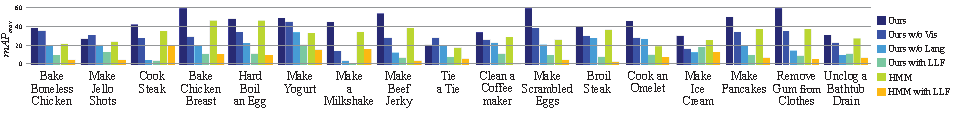
\includegraphics[width=\textwidth]{figure_10}
\vspace{-9mm}
\caption{$AP_{max}$ values for all categories, for all competing algorithms.}
\vspace{-3mm}
\label{mmAP}
\end{figure*}

Given parsing results and the ground truth, we evaluate both the quality of temporal segmentation and the activity step discovery. We base our evaluation on two widely used metrics; intersection over union ($IOU$) and mean average precision($mAP$). $\mathbf{IOU}$ measures the quality of temporal segmentation and it is defined as; $\frac{1}{N}\sum_{i=1}^N \frac{\tau^\star_i \cap \tau^\prime_{i}}{\tau^\star_i \cup \tau^\prime_{i}}$ where $N$ is the number of segments, $\tau^\star_i$ is ground truth  segment and $\tau^\prime_{i}$ is the detected segment. $\mathbf{mAP}$ is defined per activity step and can be computed based on a precision-recall curve \cite{THUMOS14}. In order to adopt these metrics into unsupervised setting, we use cluster similarity measure(csm)\cite{liao05} which enables us to use any metric in unsupervised setting. It chooses a matching of ground truth labels with predicted labels by searching over all matching and choosing the ones giving highest score. We use $mAP_{csm}$ and $IOU_{csm}$ as evaluation metrics.

\vspace{1mm}
\noindent\textbf{Accuracy of the temporal parsing.}
We compute, and plot in Figure\ref{mIOU}, the $IOU_{cms}$ values for all competing algorithms and all categories. We also average over the categories and summarize the results in the Table \ref{averM}. As the Figure~\ref{mIOU} and Table~\ref{averM} suggests, proposed method consistently outperforms the competing algorithms and its variations. One interesting observation is the importance of both modalities as a result of dramatic difference between the accuracy of our method and its single modal versions.

Moreover, the difference between our method and HMM is also significant. We believe this is due to the ill-posed definition of activities in HMM since the granularity of the activity steps is subjective. On the other hand, our method starts with the well-defined definition of finding set of steps which generate the entire collection. Hence, our algorithm do not suffer from granularity problem.
\begin{table}
\caption{Average of $IOU_{cms}$ and $mAP_{cms}$ over recipes.}
{\small
\resizebox{\columnwidth}{!}{%
\begin{tabular}{c|cc|cc|cccc}
 & KTS \cite{potapov2014category}    & KTS\cite{potapov2014category}     & HMM     & HMM    & Ours    & Ours     & Ours      & Our  \\
 &  w/ LLF &  w/ Sem &  w/ LLF &  w/Sem &  w/ LLF &  w/o Vis &  w/o Lang &  full \\
 \hline
$IOU_{cms}$  & 16.80 & 28.01      & 30.84 &   37.69   &  33.16 &  36.50 & 29.91& 52.36 \\
$mAP_{cms}$  &  n/a  & n/a        & 9.35  &   32.30   &  11.33 &  30.50 &  19.50 & 44.09 \\
\end{tabular}}}
\normalsize
\label{averM}
\vspace{-5mm}
\end{table}

\vspace{1mm}
\noindent\textbf{Coherency and accuracy of activity step discovery.}
Although $IOU_{cms}$ successfully measures the accuracy of the temporal segmentation, it can not measure the quality of discovered activities. In other words, we also need to evaluate the consistency of the activity steps detected over multiple videos. For this, we use unsupervised version of mean average precision $mAP_{cms}$. We plot the $mAP_{cms}$ values per category in Figure~\ref{mmAP} and their average over categories in Table~\ref{averM}. As the Figure~\ref{mmAP} and the Table~\ref{averM} suggests, our proposed method outperforms all competing algorithms. One interesting observation is the significant difference between semantic and low-level features. Hence, the mid-level features are key for linking multiple videos.

\vspace{1mm}
\noindent\textbf{Semantics of activity steps.}
In order to further evaluate the role of semantics, we performed a subjective analysis. We concatenated the activity step labels in the grount-truth into a label collection. Then, we ask non-expert users to choose a label for each discovered activity for each algorithm. In other words, we replaced the maximization step with subjective labels. We designed our experiments in a way that each clip received annotations from 5 different users. We randomized the ordering of videos and algorithms during the subjective evaluation. By using the activity labels provided by subjects, we compute the mean average precision wrt ground truth call it $mAP_{sem}$.

\begin{table}
\caption{Semantic mean-average-precision $mAP_{sem}$.}
{\small
\resizebox{\columnwidth}{!}{%
\begin{tabular}{c|cc|cccc}
            & HMM     & HMM    & Ours    & Ours     & Ours      & Our  \\
            & w/ LLF  &  w/Sem &  w/ LLF &  w/o Vis &  w/o Lang &  full \\ \hline
$mAP_{sem}$ & 6.44   & 24.83  &     7.28 &   28.93  &  14.83    &  39.01 \\
\end{tabular}}}
\normalsize
\vspace{-8mm}
\end{table}

Both $mAP_{cms}$ and $mAP_{sem}$ metrics suggest that our method consistently outperforms the competing ones. There is only one recipe in which our method is outperformed by our based line of no visual information. This is mostly because of the specific nature of the recipe \emph{How to tie a tie?}. In such videos the notion of object is not useful since all videos use a single object over the entire video. This single object is a \emph{tie} and does not fit the assumption of a frame based on multiple visual atoms.

\vspace{1mm}
\noindent\textbf{The importance of each modality.}
As shown in Figure~\ref{mIOU} and \ref{mmAP}, performance significantly drops when any of the modalities is ignored consistently in all categories. Hence, the joint usage is necessary. One interesting observation is the fact that using only language information performed slightly better than using only visual information. We believe this is due to the less intra-class variance in the language modality (\ie people use same words for same activities). However, it lacks many details(less complete) and more noisy than visual information. Hence these results validate the complementary nature of language and vision.

% !TEX root = recipeUnderstanding.tex


\section{Conclusions}
\vspace{-2mm}
%Discuss which recipes worked and why. Discuss the importance of semantic representation, scaling features and multi-modality.
In this paper, we try to capture the underlying structure of human communication by jointly considering visual and language cues. We experimentally validate that given a large-video collection having subtitles, it is possible to discover activities without any supervision over activities or objects. Experimental evaluation also suggests the available noisy and incomplete information is powerful enough to not only discover activities but also describe them. We also think that the resulting discovered knowledge can be effectively in many domains like multimedia interfaces and robot knowledge bases \cite{robobrain}. 
\vspace{-2mm}
\section{Acknowledgements}
\vspace{-2mm}
We acknowledge the support of ONR award N00014-13-1-0761 and ONR award N000141110389.
\vspace{-2mm}

\setlength{\tabcolsep}{1mm}
\begin{table*}
\footnotesize
\centering
\caption{Notation of the Paper}
\begin{tabular}{|cp{4cm}|cp{3cm}|cp{5cm}|}
  \hline
$y_t$ = $\left[y_t^v,y_t^l\right]$ & feature representation of $t^{th}$ frame & $I_t$ & $t^{th}$ frame of the video & $x^p_{i,r}$ & $1$ if $p^{th}$ cluster has $r^{th}$ proposal of $i^{th}$ video  \\
$x^p$ & binary vector for $p^{th}$ cluster & $L_t$ & subtitle for $t^{th}$ frame & $O^{k,k^\prime}$ & $1$ if $\#(z_t=k,z_{t^\prime})=k^\prime) = 0 \forall\quad t \leq t^\prime$ \\
$\Theta_k$ = $\left[\Theta_k^v,\Theta_k^l\right]$ & emmition prob. of $k^{th}$ activity & $z_t$ & activity ID of frame  $t$ & $f_i^k$ & $1$ if $i^{th}$ video has $k^{th}$ activity $0 o.w.$ \\
$\eta_i^{k,k^\prime}$ & $P(z_{t+1}=k^\prime|z_{t}=k)$ for $i^{th}$ vid & $\pi_i^{k,k^\prime}$ & $\eta_i^{k,k^\prime} \times f_i^k \times f_i^{k^\prime}$
& & \\ \hline
\end{tabular}
\end{table*}
\normalsize


{\small
\bibliographystyle{ieee}
\bibliography{recipeUnderstanding}
}

\end{document}
